%%%%%%%%%%%%%%%%%%%%%%%%%%%%%%%%%%%%%%%%%
% Classicthesis Typographic Thesis
% LaTeX Template
% Version 1.1 (4/8/12)
%
% This template has been downloaded from:
% http://www.LaTeXTemplates.com
%
% Original author:
% André Miede (http://www.miede.de)
%
% License:
% CC BY-NC-SA 3.0 (http://creativecommons.org/licenses/by-nc-sa/3.0/)
%
% General Tips:
% 1) Make sure to edit the classicthesis-config.file
% 2) New enumeration (A., B., C., etc in small caps): \begin{aenumerate} \end{aenumerate}
% 3) For margin notes: \marginpar or \graffito{}
% 4) Do not use bold fonts in this style, it is designed around them
% 5) Use tables as in the examples
% 6) See classicthesis-preamble.sty for useful commands
%
%%%%%%%%%%%%%%%%%%%%%%%%%%%%%%%%%%%%%%%%%

%----------------------------------------------------------------------------------------
%	PACKAGES AND OTHER DOCUMENT CONFIGURATIONS
%----------------------------------------------------------------------------------------

\documentclass[
		twoside,openright,titlepage,numbers=noenddot,headinclude,%1headlines,
                footinclude=true,cleardoublepage=empty,
                BCOR=5mm,paper=a4,fontsize=11pt, % Binding correction, paper type and font size
                ngerman,american, % Languages
                ]{scrreprt} 
                
% Includes the file which contains all the document configurations and packages - make sure to edit this file
%%%%%%%%%%%%%%%%%%%%%%%%%%%%%%%%%%%%%%%%%
% Thesis Configuration File
%
% The main lines to change in this file are in the DOCUMENT VARIABLES
% section, the rest of the file is for advanced configuration.
%
%%%%%%%%%%%%%%%%%%%%%%%%%%%%%%%%%%%%%%%%%

%----------------------------------------------------------------------------------------
%	DOCUMENT VARIABLES
%	Fill in the lines below to enter your information into the thesis template
%	Each of the commands can be cited anywhere in the thesis
%----------------------------------------------------------------------------------------

% Remove drafting to get rid of the '[ Date - classicthesis version 4.0 ]' text at the bottom of every page
\PassOptionsToPackage{eulerchapternumbers,listings,drafting, pdfspacing, subfig,beramono,eulermath,parts}{classicthesis}
% Available options: drafting parts nochapters linedheaders eulerchapternumbers beramono eulermath pdfspacing minionprospacing tocaligned dottedtoc manychapters listings floatperchapter subfig
% Adding 'dottedtoc' will make page numbers in the table of contents flushed right with dots leading to them

\newcommand{\myTitle}{A Classic Thesis Style\xspace}
\newcommand{\mySubtitle}{An Homage to The Elements of Typographic Style\xspace}
\newcommand{\myDegree}{Doktor-Ingenieur (Dr.-Ing.)\xspace}
\newcommand{\myName}{Andr\'e Miede\xspace}
\newcommand{\myProf}{Put name here\xspace}
\newcommand{\myOtherProf}{Put name here\xspace}
\newcommand{\mySupervisor}{Put name here\xspace}
\newcommand{\myFaculty}{Put data here\xspace}
\newcommand{\myDepartment}{Put data here\xspace}
\newcommand{\myUni}{Put data here\xspace}
\newcommand{\myLocation}{Darmstadt\xspace}
\newcommand{\myTime}{December 2011\xspace}
\newcommand{\myVersion}{version 4.0\xspace}

%----------------------------------------------------------------------------------------
%	USEFUL COMMANDS
%----------------------------------------------------------------------------------------

\newcommand{\ie}{i.\,e.}
\newcommand{\Ie}{I.\,e.}
\newcommand{\eg}{e.\,g.}
\newcommand{\Eg}{E.\,g.} 

\newcounter{dummy} % Necessary for correct hyperlinks (to index, bib, etc.)
\providecommand{\mLyX}{L\kern-.1667em\lower.25em\hbox{Y}\kern-.125emX\@}

%----------------------------------------------------------------------------------------
%	PACKAGES
%----------------------------------------------------------------------------------------

\usepackage{lipsum} % Used for inserting dummy 'Lorem ipsum' text into the template

%------------------------------------------------
 
\PassOptionsToPackage{latin9}{inputenc} % latin9 (ISO-8859-9) = latin1+"Euro sign"
\usepackage{inputenc}
 
 %------------------------------------------------

%\PassOptionsToPackage{ngerman,american}{babel}  % Change this to your language(s)
% Spanish languages need extra options in order to work with this template
%\PassOptionsToPackage{spanish,es-lcroman}{babel}
\usepackage{babel}

%------------------------------------------------			

\PassOptionsToPackage{square,numbers}{natbib}
 \usepackage{natbib}
 
 %------------------------------------------------

\PassOptionsToPackage{fleqn}{amsmath} % Math environments and more by the AMS 
 \usepackage{amsmath}
 
 %------------------------------------------------

\PassOptionsToPackage{T1}{fontenc} % T2A for cyrillics
\usepackage{fontenc}

%------------------------------------------------

\usepackage{xspace} % To get the spacing after macros right

%------------------------------------------------

\usepackage{mparhack} % To get marginpar right

%------------------------------------------------

\usepackage{fixltx2e} % Fixes some LaTeX stuff 

%------------------------------------------------

\PassOptionsToPackage{smaller}{acronym} % Include printonlyused in the first bracket to only show acronyms used in the text
\usepackage{acronym} % nice macros for handling all acronyms in the thesis

%------------------------------------------------

%\renewcommand*{\acsfont}[1]{\textssc{#1}} % For MinionPro
\renewcommand{\bflabel}[1]{{#1}\hfill} % Fix the list of acronyms

%------------------------------------------------

\PassOptionsToPackage{pdftex}{graphicx}
\usepackage{graphicx} 

%----------------------------------------------------------------------------------------
%	FLOATS: TABLES, FIGURES AND CAPTIONS SETUP
%----------------------------------------------------------------------------------------

\usepackage{tabularx} % Better tables
\setlength{\extrarowheight}{3pt} % Increase table row height
\newcommand{\tableheadline}[1]{\multicolumn{1}{c}{\spacedlowsmallcaps{#1}}}
\newcommand{\myfloatalign}{\centering} % To be used with each float for alignment
\usepackage{caption}
\captionsetup{format=hang,font=small}
\usepackage{subfig}  

%----------------------------------------------------------------------------------------
%	CODE LISTINGS SETUP
%----------------------------------------------------------------------------------------

\usepackage{listings} 
%\lstset{emph={trueIndex,root},emphstyle=\color{BlueViolet}}%\underbar} % for special keywords
\lstset{language=[LaTeX]Tex, % Specify the language for listings here
keywordstyle=\color{RoyalBlue}, % Add \bfseries for bold
basicstyle=\small\ttfamily, % Makes listings a smaller font size and a different font
%identifierstyle=\color{NavyBlue}, % Color of text inside brackets
commentstyle=\color{Green}\ttfamily, % Color of comments
stringstyle=\rmfamily, % Font type to use for strings
numbers=left, % Change left to none to remove line numbers
numberstyle=\scriptsize, % Font size of the line numbers
stepnumber=5, % Increment of line numbers
numbersep=8pt, % Distance of line numbers from code listing
showstringspaces=false, % Sets whether spaces in strings should appear underlined
breaklines=true, % Force the code to stay in the confines of the listing box
%frameround=ftff, % Uncomment for rounded frame
frame=single, % Frame border - none/leftline/topline/bottomline/lines/single/shadowbox/L
belowcaptionskip=.75\baselineskip % Space after the "Listing #: Desciption" text and the listing box
}

%----------------------------------------------------------------------------------------
%	HYPERREFERENCES
%----------------------------------------------------------------------------------------

\PassOptionsToPackage{pdftex,hyperfootnotes=false,pdfpagelabels}{hyperref}
\usepackage{hyperref}  % backref linktocpage pagebackref
\pdfcompresslevel=9
\pdfadjustspacing=1

\hypersetup{
% Uncomment the line below to remove all links (to references, figures, tables, etc)
%draft, 
colorlinks=true, linktocpage=true, pdfstartpage=3, pdfstartview=FitV,
% Uncomment the line below if you want to have black links (e.g. for printing black and white)
%colorlinks=false, linktocpage=false, pdfborder={0 0 0}, pdfstartpage=3, pdfstartview=FitV, 
breaklinks=true, pdfpagemode=UseNone, pageanchor=true, pdfpagemode=UseOutlines,
plainpages=false, bookmarksnumbered, bookmarksopen=true, bookmarksopenlevel=1,
hypertexnames=true, pdfhighlight=/O, urlcolor=webbrown, linkcolor=RoyalBlue, citecolor=webgreen,
%------------------------------------------------
% PDF file meta-information
pdftitle={\myTitle},
pdfauthor={\textcopyright\ \myName, \myUni, \myFaculty},
pdfsubject={},
pdfkeywords={},
pdfcreator={pdfLaTeX},
pdfproducer={LaTeX with hyperref and classicthesis}
%------------------------------------------------
}   

%----------------------------------------------------------------------------------------
%	BACKREFERENCES
%----------------------------------------------------------------------------------------

\usepackage{ifthen} % Allows the user of the \ifthenelse command
\newboolean{enable-backrefs} % Variable to enable backrefs in the bibliography
\setboolean{enable-backrefs}{false} % Variable value: true or false

\newcommand{\backrefnotcitedstring}{\relax} % (Not cited.)
\newcommand{\backrefcitedsinglestring}[1]{(Cited on page~#1.)}
\newcommand{\backrefcitedmultistring}[1]{(Cited on pages~#1.)}
\ifthenelse{\boolean{enable-backrefs}} % If backrefs were enabled
{
\PassOptionsToPackage{hyperpageref}{backref}
\usepackage{backref} % to be loaded after hyperref package 
\renewcommand{\backreftwosep}{ and~} % separate 2 pages
\renewcommand{\backreflastsep}{, and~} % separate last of longer list
\renewcommand*{\backref}[1]{}  % disable standard
\renewcommand*{\backrefalt}[4]{% detailed backref
\ifcase #1 
\backrefnotcitedstring
\or
\backrefcitedsinglestring{#2}
\else
\backrefcitedmultistring{#2}
\fi}
}{\relax} 

%----------------------------------------------------------------------------------------
%	AUTOREFERENCES SETUP
%	Redefines how references in text are prefaced for different 
%	languages (e.g. "Section 1.2" or "section 1.2")
%----------------------------------------------------------------------------------------

\makeatletter
\@ifpackageloaded{babel}
{
\addto\extrasamerican{
\renewcommand*{\figureautorefname}{Figure}
\renewcommand*{\tableautorefname}{Table}
\renewcommand*{\partautorefname}{Part}
\renewcommand*{\chapterautorefname}{Chapter}
\renewcommand*{\sectionautorefname}{Section}
\renewcommand*{\subsectionautorefname}{Section}
\renewcommand*{\subsubsectionautorefname}{Section}
}
\addto\extrasngerman{
\renewcommand*{\paragraphautorefname}{Absatz}
\renewcommand*{\subparagraphautorefname}{Unterabsatz}
\renewcommand*{\footnoteautorefname}{Fu\"snote}
\renewcommand*{\FancyVerbLineautorefname}{Zeile}
\renewcommand*{\theoremautorefname}{Theorem}
\renewcommand*{\appendixautorefname}{Anhang}
\renewcommand*{\equationautorefname}{Gleichung}
\renewcommand*{\itemautorefname}{Punkt}
}
\providecommand{\subfigureautorefname}{\figureautorefname} % Fix to getting autorefs for subfigures right
}{\relax}
\makeatother

%----------------------------------------------------------------------------------------

\usepackage{classicthesis} 

%----------------------------------------------------------------------------------------
%	CHANGING TEXT AREA 
%----------------------------------------------------------------------------------------

%\linespread{1.05} % a bit more for Palatino
%\areaset[current]{312pt}{761pt} % 686 (factor 2.2) + 33 head + 42 head \the\footskip
%\setlength{\marginparwidth}{7em}%
%\setlength{\marginparsep}{2em}%

%----------------------------------------------------------------------------------------
%	USING DIFFERENT FONTS
%----------------------------------------------------------------------------------------

%\usepackage[oldstylenums]{kpfonts} % oldstyle notextcomp
%\usepackage[osf]{libertine}
%\usepackage{hfoldsty} % Computer Modern with osf
%\usepackage[light,condensed,math]{iwona}
%\renewcommand{\sfdefault}{iwona}
%\usepackage{lmodern} % <-- no osf support :-(
%\usepackage[urw-garamond]{mathdesign} <-- no osf support :-(

\begin{document}

\frenchspacing % Reduces space after periods to make text more compact

\raggedbottom % Makes all pages the height of the text on that page

\selectlanguage{american} % Select your default language - e.g. american or ngerman

%\renewcommand*{\bibname}{new name} % Uncomment to change the name of the bibliography
%\setbibpreamble{} % Uncomment to include a preamble to the bibliography - some text before the reference list starts

\pagenumbering{roman} % Roman page numbering prior to the start of the thesis content (i, ii, iii, etc)

\pagestyle{plain} % Suppress headers for the pre-content pages

%----------------------------------------------------------------------------------------
%	PRE-CONTENT THESIS PAGES
%----------------------------------------------------------------------------------------

% Title Page

\begin{titlepage}

% \begin{addmargin}[-1cm]{-3cm}
\begin{center}
\large

\hfill
\vfill

\begingroup
\color{Maroon}\spacedallcaps{\myTitle} \\ \bigskip % Thesis title
\endgroup

\spacedlowsmallcaps{\myName} % Your name

\vfill

%
\includegraphics[width=6cm]{gfx/TFZsuperellipse_bw} \\ \medskip % Picture

\mySubtitle \\ \medskip % Thesis subtitle
%\myDegree \\
\myDepartment \\
%\myFaculty \\
\myUni \\ \bigskip

\myTime\ %-- \myVersion % Time and version

\vfill

\end{center}
% \end{addmargin}

\end{titlepage} % Main title page

% Back of the title page

\thispagestyle{empty}

\hfill

\vfill

\noindent\myName: \textit{\myTitle,} \mySubtitle, %\myDegree, 
\textcopyright\ \myTime

% You may wish to do something with the back of the title page, such as including your supervisors, location or time frame of the work. Below is an example of doing so although you may want to tweak it to your liking.

%\bigskip

%\noindent\spacedlowsmallcaps{Supervisors}: \\
%\myProf \\
%\myOtherProf \\ 
%\mySupervisor

%\medskip \\

%\noindent\spacedlowsmallcaps{Location}: \\
%\myLocation

%\medskip \\

%\noindent\spacedlowsmallcaps{Time Frame}: \\
%\myTime
 % Back of the title page

\cleardoublepage% Dedication

\thispagestyle{empty}
\refstepcounter{dummy}

\pdfbookmark[1]{Dedication}{Dedication} % Bookmark name visible in a PDF viewer

\vspace*{3cm}

\begin{center}
\emph{Ohana} means family. \\
Family means nobody gets left behind, or forgotten. \\ \medskip
--- Lilo \& Stitch    
\end{center}

\medskip

\begin{center}
Dedicated to the loving memory of Rudolf Miede. \\ \smallskip
1939\,--\,2005
\end{center} % Dedication page

%\cleardoublepage\include{FrontBackMatter/Foreword} % Uncomment and create a Foreword.tex to include a foreword

\cleardoublepage% Abstract

\pdfbookmark[1]{Abstract}{Abstract} % Bookmark name visible in a PDF viewer

\begingroup
\let\clearpage\relax
\let\cleardoublepage\relax
\let\cleardoublepage\relax

\chapter*{Abstract} % Abstract name

INTEGRAL, the International Gamma Ray Astrophysics Laboratory, is a satellite launched in 2002. Containing four primary instruments, INTEGRAL looks at sources in energy ranges approximately between 5 keV and 10 MeV, from hard X-rays to Gamma rays. 

The INTEGRAL archive contains data for many sources that have not been fully explored. This project focuses on a sample of High Mass X-ray Binary sources including some thought to have eclipses or long term periodic variability. Lomb-Scarge spectral analysis and Phase Dispersion Minimisation is used to find periodicities in the light curves of these sources, and broadly categorise them into the 3 main classes of HXMB, the Supergiant X-ray Binaries, Superfast X-ray Transients, and Be Star X-ray Binaries. The project also discusses the utility of the methods used in finding periodicities in these sources. 



\endgroup			

\vfill % Abstract page

\cleardoublepage% Publications - a page listing research articles written using content in the thesis

\pdfbookmark[1]{Publications}{Publications} % Bookmark name visible in a PDF viewer

\chapter*{Publications} % Publications page text

Some ideas and figures have appeared previously in the following publications:

\bigskip

\noindent Put your publications from the thesis here. The packages \texttt{multibib} or \texttt{bibtopic} etc. can be used to handle multiple different bibliographies in your document. % Publications from the thesis page

\cleardoublepage% Acknowledgements

\pdfbookmark[1]{Acknowledgements}{Acknowledgements} % Bookmark name visible in a PDF viewer

\begin{flushright}{\slshape    
We have seen that computer programming is an art, \\ 
because it applies accumulated knowledge to the world, \\ 
because it requires skill and ingenuity, and especially \\
because it produces objects of beauty.} \\ \medskip
--- \defcitealias{knuth:1974}{Donald E. Knuth}\citetalias{knuth:1974} \citep{knuth:1974}
\end{flushright}

\bigskip

%----------------------------------------------------------------------------------------

\begingroup

\let\clearpage\relax
\let\cleardoublepage\relax
\let\cleardoublepage\relax

\chapter*{Acknowledgements} % Acknowledgements section text

Put your acknowledgements here.\\

\noindent Many thanks to everybody who already sent me a postcard!\\

\noindent Regarding the typography and other help, many thanks go to Marco Kuhlmann, Philipp Lehman, Lothar Schlesier, Jim Young, Lorenzo Pantieri and Enrico Gregorio\footnote{Members of GuIT (Gruppo Italiano Utilizzatori di \TeX\ e \LaTeX )}, J\"org Sommer, Joachim K\"ostler, Daniel Gottschlag, Denis Aydin, Paride Legovini, Steffen Prochnow, Nicolas Repp, Hinrich Harms, Roland Winkler,  and the whole \LaTeX-community for support, ideas and some great software.

\bigskip

\noindent\emph{Regarding \mLyX}: The \mLyX\ port was intially done by
\emph{Nicholas Mariette} in March 2009 and continued by
\emph{Ivo Pletikosi\'c} in 2011. Thank you very much for your work and the contributions to the original style.

\endgroup % Acknowledgements page

\pagestyle{scrheadings} % Show chapter titles as headings

\cleardoublepage% Table of Contents - List of Tables/Figures/Listings and Acronyms

\refstepcounter{dummy}

\pdfbookmark[1]{\contentsname}{tableofcontents} % Bookmark name visible in a PDF viewer

\setcounter{tocdepth}{2} % Depth of sections to include in the table of contents - currently up to subsections

\setcounter{secnumdepth}{3} % Depth of sections to number in the text itself - currently up to subsubsections

\manualmark
\markboth{\spacedlowsmallcaps{\contentsname}}{\spacedlowsmallcaps{\contentsname}}
\tableofcontents 
\automark[section]{chapter}
\renewcommand{\chaptermark}[1]{\markboth{\spacedlowsmallcaps{#1}}{\spacedlowsmallcaps{#1}}}
\renewcommand{\sectionmark}[1]{\markright{\thesection\enspace\spacedlowsmallcaps{#1}}}

\clearpage

\begingroup 
\let\clearpage\relax
\let\cleardoublepage\relax
\let\cleardoublepage\relax

%----------------------------------------------------------------------------------------
%	List of Figures
%----------------------------------------------------------------------------------------

\refstepcounter{dummy}
%\addcontentsline{toc}{chapter}{\listfigurename} % Uncomment if you would like the list of figures to appear in the table of contents
\pdfbookmark[1]{\listfigurename}{lof} % Bookmark name visible in a PDF viewer

\listoffigures

\vspace*{8ex}
\newpage

%----------------------------------------------------------------------------------------
%	List of Tables
%----------------------------------------------------------------------------------------

\refstepcounter{dummy}
%\addcontentsline{toc}{chapter}{\listtablename} % Uncomment if you would like the list of tables to appear in the table of contents
\pdfbookmark[1]{\listtablename}{lot} % Bookmark name visible in a PDF viewer

\listoftables
        
\vspace*{8ex}
\newpage
    
%----------------------------------------------------------------------------------------
%	List of Listings
%---------------------------------------------------------------------------------------- 

\refstepcounter{dummy}
%\addcontentsline{toc}{chapter}{\lstlistlistingname} % Uncomment if you would like the list of listings to appear in the table of contents
\pdfbookmark[1]{\lstlistlistingname}{lol} % Bookmark name visible in a PDF viewer

\lstlistoflistings 

\vspace*{8ex}
\newpage
       
%----------------------------------------------------------------------------------------
%	Acronyms
%----------------------------------------------------------------------------------------

\refstepcounter{dummy}
%\addcontentsline{toc}{chapter}{Acronyms} % Uncomment if you would like the acronyms to appear in the table of contents
\pdfbookmark[1]{Acronyms}{acronyms} % Bookmark name visible in a PDF viewer

\markboth{\spacedlowsmallcaps{Acronyms}}{\spacedlowsmallcaps{Acronyms}}

\chapter*{Acronyms}

\begin{acronym}[UML]
\acro{DRY}{Don't Repeat Yourself}
\acro{API}{Application Programming Interface}
\acro{UML}{Unified Modeling Language}
\end{acronym}  
                   
\endgroup

\cleardoublepage % Contents, list of figures/tables/listings and acronyms

\pagenumbering{arabic} % Arabic page numbering for thesis content (1, 2, 3, etc)
%\setcounter{page}{90} % Uncomment to manually start the page counter at an arbitrary value (for example if you wish to count the pre-content pages in the page count)

\cleardoublepage % Avoids problems with pdfbookmark

%----------------------------------------------------------------------------------------
%	THESIS CONTENT - CHAPTERS
%----------------------------------------------------------------------------------------

\ctparttext{You can put some informational part preamble text here. Illo principalmente su nos. Non message \emph{occidental} angloromanic da. Debitas effortio simplificate sia se, auxiliar summarios da que, se avantiate publicationes via. Pan in terra summarios, capital interlingua se que. Al via multo esser specimen, campo responder que da. Le usate medical addresses pro, europa origine sanctificate nos se.} % Text on the Part 1 page describing  the content in Part 1

\part{Some Kind of Manual} % First part of the thesis

% Chapter 1

\chapter{Introduction} % Chapter title

\label{ch:introduction} % For referencing the chapter elsewhere, use \autoref{ch:introduction} 

%----------------------------------------------------------------------------------------

This template for \LaTeX\ has two goals:
\begin{enumerate}
\item Provide students with an easy-to-use template for their Master's or PhD thesis (though it might also be used by other types of authors for reports, books, etc.).
\item Provide a classic, high-quality typographic style that is inspired by \citeauthor{bringhurst:2002}'s ``\emph{The Elements of Typographic Style}'' \citep{bringhurst:2002}.
\marginpar{\myTitle \myVersion}
\end{enumerate}

The bundle is configured to run with a \emph{full} MiK\TeX\ or \TeX Live installation right away and, therefore, it uses only freely available fonts.

People interested only in the nice style and not the whole bundle can now use the style stand-alone via the file \texttt{classicthesis.sty}. This works now also with ``plain'' \LaTeX.

As of version 3.0, \texttt{classicthesis} can also be easily used with \mLyX\footnote{\url{http://www.lyx.org}} thanks to Nicholas Mariette and Ivo Pletikosi\'c. The \mLyX\ version of this manual will contain more information on the details.

This should enable anyone with a basic knowledge of \LaTeXe\ or \mLyX\ to produce beautiful documents without too much effort. In the end, this is my overall goal: more beautiful documents, especially theses, as I am tired of seeing so many ugly ones.

The whole template and the used style is released under the \textsmaller{GNU} General Public License. 

If you like the style then I would appreciate a postcard:
\begin{center}
Andre Miede \\
Detmolder Strasse 32 \\
31737 Rinteln \\
Germany
\end{center}

\noindent The postcards I received so far are available at:
\begin{center}
 \url{http://postcards.miede.de}
\end{center}
\marginpar{A well-balanced line width improves the legibility of the text. That's what typography is all about, right?} So far, many theses, some books, and several other publications have been typeset successfully with it. If you are interested in some typographic details behind it, enjoy Robert Bringhurst's wonderful book. % \citep{bringhurst:2002}.

\paragraph{Important Note:} Some things of this style might look unusual at first glance, many people feel so in the beginning. However, all things are intentionally designed to be as they are, especially these:
\begin{itemize}
\item No bold fonts are used. Italics or spaced small caps do the job quite well.
\item The size of the text body is intentionally shaped like it is. It supports both legibility and allows a reasonable amount of information to be on a page. And, no: the lines are not too short.
\item The tables intentionally do not use vertical or double rules. See the documentation for the \texttt{booktabs} package for a nice discussion of this topic.\footnote{To be found online at \\ \url{http://www.ctan.org/tex-archive/macros/latex/contrib/booktabs/}.}
\item And last but not least, to provide the reader with a way easier access to page numbers in the table of contents, the page numbers are right behind the titles. Yes, they are \emph{not} neatly aligned at the right side and they are \emph{not} connected with dots that help the eye to bridge a distance that is not necessary. If you are still not convinced: is your reader interested in the page number or does she want to sum the numbers up?
\end{itemize}

\noindent Therefore, please do not break the beauty of the style by changing these things unless you really know what you are doing! Please.

%----------------------------------------------------------------------------------------

\section{Organization}
A very important factor for successful thesis writing is the organization of the material. This template suggests a structure as the following:
\begin{itemize}
\marginpar{You can use these margins for summaries of the text body\dots}
\item\texttt{Chapters/} is where all the ``real'' content goes in separate files such as \texttt{Chapter01.tex} etc.
\item\texttt{FrontBackMatter/} is where all the stuff goes that surrounds the ``real'' content, such as the acknowledgments, dedication, etc.
\item\texttt{gfx/} is where you put all the graphics you use in the thesis. Maybe they should be organized into subfolders depending on the chapter they are used in, if you have a lot of graphics.
\item\texttt{Bibliography.bib}: the Bib\TeX\ database to organize all the references you might want to cite.
\item\texttt{classicthesis.sty}: the style definition to get this awesome look and feel. Bonus: works with both \LaTeX\ and \textsc{pdf}\LaTeX\dots and \mLyX.
\item\texttt{ClassicThesis.tcp} a \TeX nicCenter project file. Great tool and it's free!
\item\texttt{ClassicThesis.tex}: the main file of your thesis where all the content gets bundled together.
\item\texttt{classicthesis-config.tex}: a central place to load all nifty packages that are used. In there, you can also activate backrefs in order to have information in the bibliography about where a source was cited in the text (\ie, the page number).
    
\emph{Make your changes and adjustments here.} This means that you specify here the options you want to load \texttt{classicthesis.sty} with. You also adjust the title of your thesis, your name, and all similar information here. Refer to \autoref{sec:custom} for more information.

This had to change as of version 3.0 in order to enable an easy transition from the ``basic'' style to \mLyX.
\end{itemize}

\noindent In total, this should get you started in no time.

%----------------------------------------------------------------------------------------

\section{Style Options}\label{sec:options}

There are a couple of options for \texttt{classicthesis.sty} that allow for a bit of freedom concerning the layout: \marginpar{\dots or your supervisor might use the margins for some comments of her own while reading.}
\begin{itemize}
\item General:
\begin{itemize}
\item\texttt{drafting}: prints the date and time at the bottom of each page, so you always know which version you are dealing with. Might come in handy not to give your Prof. that old draft.
\end{itemize}
	
\item Parts and Chapters:
\begin{itemize}
\item\texttt{parts}: if you use Part divisions for your document, you should choose this option. (Cannot be used together with \texttt{nochapters}.)

\item\texttt{nochapters}: allows to use the look-and-feel with classes that do not use chapters, \eg, for articles. Automatically turns off a couple of other options: \texttt{eulerchapternumbers}, \texttt{linedheaders}, \texttt{listsseparated}, and \texttt{parts}. 

\item\texttt{linedheaders}: changes the look of the chapter headings a bit by adding a horizontal line above the chapter title. The chapter number will also be moved to the top of the page, above the chapter title.
\end{itemize}

\item Typography:
\begin{itemize}
\item\texttt{eulerchapternumbers}: use figures from Hermann Zapf's Euler math font for the chapter numbers. By default, old style figures from the Palatino font are used.

\item\texttt{beramono}: loads Bera Mono as typewriter font. (Default setting is using the standard CM typewriter font.)
\item\texttt{eulermath}: loads the awesome Euler fonts for math. (Palatino is used as default font.)

\item\texttt{pdfspacing}: makes use of pdftex' letter spacing capabilities via the \texttt{microtype} package.\footnote{Use \texttt{microtype}'s \texttt{DVIoutput} option to generate DVI with pdftex.} This fixes some serious issues regarding math formul\ae\ etc. (\eg, ``\ss'') in headers. 

\item\texttt{minionprospacing}: uses the internal \texttt{textssc} command of the \texttt{MinionPro} package for letter spacing. This automatically enables the \texttt{minionpro} option and overrides the \texttt{pdfspacing} option.
\end{itemize}  

\item Table of Contents:
\begin{itemize}
\item\texttt{tocaligned}: aligns the whole table of contents on the left side. Some people like that, some don't.

\item\texttt{dottedtoc}: sets pagenumbers flushed right in the table of contents.

\item\texttt{manychapters}: if you need more than nine chapters for your document, you might not be happy with the spacing between the chapter number and the chapter title in the Table of Contents. This option allows for additional space in this context. However, it does not look as ``perfect'' if you use \verb|\parts| for structuring your document.
\end{itemize}

\item Floats:
\begin{itemize}
\item\texttt{listings}: loads the \texttt{listings} package (if not already done) and configures the List of Listings accordingly.
    
\item\texttt{floatperchapter}: activates numbering per chapter for all floats such as figures, tables, and listings (if used).	
    
\item\texttt{subfig}(\texttt{ure}): is passed to the \texttt{tocloft} package to enable compatibility with the \texttt{subfig}(\texttt{ure}) package. Use this option if you want use classicthesis with the \texttt{subfig} package.

\end{itemize}    

\end{itemize}

\noindent The best way to figure these options out is to try the different possibilities and see, what you and your supervisor like best.

In order to make things easier in general, \texttt{classicthesis-config.tex} contains some useful commands that might help you.

%----------------------------------------------------------------------------------------

\section{Customization}\label{sec:custom}

This section will give you some hints about how to adapt \texttt{classicthesis} to your needs.

The file \texttt{classicthesis.sty} contains the core functionality of the style and in most cases will be left intact, whereas the file \texttt{classic\-thesis-config.tex} is used for some common user customizations. 

The first customization you are about to make is to alter the document title, author name, and other thesis details. In order to do this, replace the data in the following lines of \texttt{classicthesis-config.tex:}\marginpar{Modifications in \texttt{classic\-thesis-config.tex}
}

\begin{lstlisting}[frame=lt]
\newcommand{\myTitle}{A Classic Thesis Style\xspace}
\newcommand{\mySubtitle}{An Homage to ...\xspace}
\newcommand{\myDegree}{Doktor-Ingenieur (Dr.-Ing.)\xspace}
\end{lstlisting}

Further customization can be made in \texttt{classicthesis-config.tex} by choosing the options to \texttt{classicthesis.sty} (see~\autoref{sec:options}) in a line that looks like this:

\begin{lstlisting}[frame=lt]
\PassOptionsToPackage{eulerchapternumbers,listings,drafting, pdfspacing, subfig,beramono,eulermath,parts}{classicthesis}

\end{lstlisting}

If you want to use backreferences from your citations to the pages they were cited on, change the following line from:
\begin{lstlisting}[breaklines=false,frame=lt]
\setboolean{enable-backrefs}{false}
\end{lstlisting}
to
\begin{lstlisting}[breaklines=false,frame=lt]
\setboolean{enable-backrefs}{true}
\end{lstlisting}

Many other customizations in \texttt{classicthesis-config.tex} are possible, but you should be careful making changes there, since some changes could cause errors.

Finally, changes can be made in the file \texttt{classicthesis.sty}, \marginpar{Modifications in \texttt{classicthesis.sty}} although this is mostly not designed for user customization. The main change that might be made here is the text-block size, for example, to get longer lines of text.

%----------------------------------------------------------------------------------------

\section{Issues}\label{sec:issues}
This section will list some information about problems using \texttt{classic\-thesis} in general or using it with other packages.

Beta versions of \texttt{classicthesis} can be found at the following Google code repository:
\begin{center}
\url{http://code.google.com/p/classicthesis/}
\end{center}

\noindent There, you can also post serious bugs and problems you encounter.

\subsection*{Compatibility with the \texttt{glossaries} Package}
If you want to use the \texttt{glossaries} package, take care of loading it with the following options:
\begin{verbatim}
\usepackage[style=long,nolist]{glossaries}
\end{verbatim}

\noindent Thanks to Sven Staehs for this information. 

\subsection*{Compatibility with the (Spanish) \texttt{babel} Package}
Spanish languages need an extra option in order to work with this template:
\begin{verbatim}
\usepackage[spanish,es-lcroman]{babel}
\end{verbatim}

\noindent Thanks to an unknown person for this information (via Google Code issue reporting). 

\subsection*{Compatibility with the \texttt{pdfsync} Package}
Using the \texttt{pdfsync} package leads to linebreaking problems with the \texttt{graffito} command. Thanks to Henrik Schumacher for this information. 

%----------------------------------------------------------------------------------------

\section{Future Work}
So far, this is a quite stable version that served a couple of people well during their thesis time. However, some things are still not as they should be. Proper documentation in the standard format is still missing. In the long run, the style should probably be published separately, with the template bundle being only an application of the style. Alas, there is no time for that at the moment\dots it could be a nice task for a small group of \LaTeX nicians.

Please do not send me email with questions concerning \LaTeX\ or the template, as I do not have time for an answer. But if you have comments, suggestions, or improvements for the style or the template in general, do not hesitate to write them on that postcard of yours.

%----------------------------------------------------------------------------------------

\section{License}
\paragraph{GNU General Public License:} This program is free software; you can redistribute it and/or modify it under the terms of the \textsmaller{GNU} General Public License as published by the Free Software Foundation; either version 2 of the License, or (at your option) any later version.

This program is distributed in the hope that it will be useful, but \emph{without any warranty}; without even the implied warranty of \emph{merchantability} or \emph{fitness for a particular purpose}. See the \textsmaller{GNU} General Public License for more details. % Chapter 1

\cleardoublepage % Empty page before the start of the next part

%------------------------------------------------

\ctparttext{You can put some informational part preamble text here. Illo principalmente su nos. Non message \emph{occidental} angloromanic da. Debitas effortio simplificate sia se, auxiliar summarios da que, se avantiate publicationes via. Pan in terra summarios, capital interlingua se que. Al via multo esser specimen, campo responder que da. Le usate medical addresses pro, europa origine sanctificate nos se.} % Text on the Part 2 page describing the content in Part 2

\part{The Showcase} % Second part of the thesis

% Chapter 2

\chapter{Introduction} % Chapter title

\label{ch:introduction} % For referencing the chapter elsewhere, use \autoref{ch:introduction} 

%----------------------------------------------------------------------------------------

\section{X-ray Sources}


\subsection{High Mass X-ray Binaries} % Chapter 2
% Chapter 3

\chapter{Methodology} % Chapter title

\label{ch:method} % For referencing the chapter elsewhere, use \autoref{ch:introduction} 

%----------------------------------------------------------------------------------------
\section{Project Objectives}
The project aims to:
\begin{itemize}
\item Plot and visualise the light curves from the INTEGRAL data for the sample of sources.
\item Visualise the orbital light curves for the sources.
\item Compare the Superfast X-ray Transient sources with both Be star X-ray Binaries and Supergiant X-ray Binaries. 
\item Examine the eclipse profiles of those sources exhibiting them.
\end{itemize}
In order to achieve these aims it is necessary to have the tools to be able to produce a selection of results from the data. Chosen for familiarity and ease of use, Python was used as the programming language to produce the scripts and tools to analyse the data. The project used a standard build of Python 2.7, as well as additional libraries. Matplotlib was used to produce plots and graphs. Numpy and Scipy were used for their broad selection of tools that aid scientific computing.

\section{Test Source}
A large focus of the project was producing and testing the code for data analysis. Approximately half of the time spend during the year was spent testing and bug fixing. IGR J18027-2016 was selected as a test source. This source is a SGXB where the compact object is a neutron star that is accreting from a B giant. It is a particularly bright object, and also has a regular eclipse, which makes the source ideal for testing Lomb-Scargle period analysis, a key tool in the project. 

\section{Aims}
The code needs to perform the following:
\begin{itemize}
\item Read in the data from a text file.
\item Filter the data.
\item Re-bin the data into larger bins. Typically these will be approximately a day to a month. This then needs to be plotted.
\item Find periodicities in the data using the Lomb-Scarge method and produce a periodogram.
\item Additionally use Phase Dispersion Minimisation as a method of finding periods, and produce a graph of the result.
\item Fold the light curve on a given period, and re-bin. Then plot a folded lightcurve for a source.
\item Quantify errors for all these calculations.
\end{itemize}

\section{Reading in Data}
The starting point for the workflow is a text file containing the data. Data points are lines in the file. The Numpy module provides a convenient function for reading from text files, loadtxt, which can be used to read a file into an array. The function can also \textquotedblleft{}unpack\textquotedblright{} the data, outputting the data column-wise.  It is changed to have the data as a list of rows, so that the entire data set can be iterated over by simply looping over all rows.

\section{Filtering the Data}
When viewing data collected by the IBIS/ISGRI instrument, the data is typically very noisy. The INTEGRAL satellite has been operational for ten years, and so light curves for some sources are particularly good if the source is in an area of the sky that the satellite frequently points to. However some observations, science windows, have particularly large standard errors, often a magnitude larger than the flux reading. This can be caused by two features of the INTEGRAL satellite. 

Firstly, as the INTEGRAL satellite sweeps through the plane of the sky, sources are observed that the satellite does not directly point at. When a source is observed where it is at the edge of the field of view of the instrumentation, it typically has a much higher standard error. This is a feature of the coded mask aperture that is used for imaging; they perform best when pointing directly at a source. Science windows where the source is measured with an off axis angle greater than 12 \textdegree{} are removed. 

Secondly, the exposure time for a typical science window is around 20 minutes.  Sometimes the instruments will record an exposure that was much shorter, and these measurements also have a much higher standard error. Data points with an exposure time shorter than 500 s are removed. 

Initially during testing and developing of the project code, when filtering was not implemented, the Lomb-Scargle period analysis had difficulty finding the strong periodicity in the test source. This is because although other parts of the code output binned data, where an average weighted by the standard error on the flux has been used, the Lomb-Scargle routine does not use this, instead running on the raw lightcurve, and so extreme data points lower the visibility of the peak in the periodogram. For sources which show a weaker signal in their periodogram, this is crucial to being able to identify the correct peak to fold on.

\begin{figure}[h!]
\centering
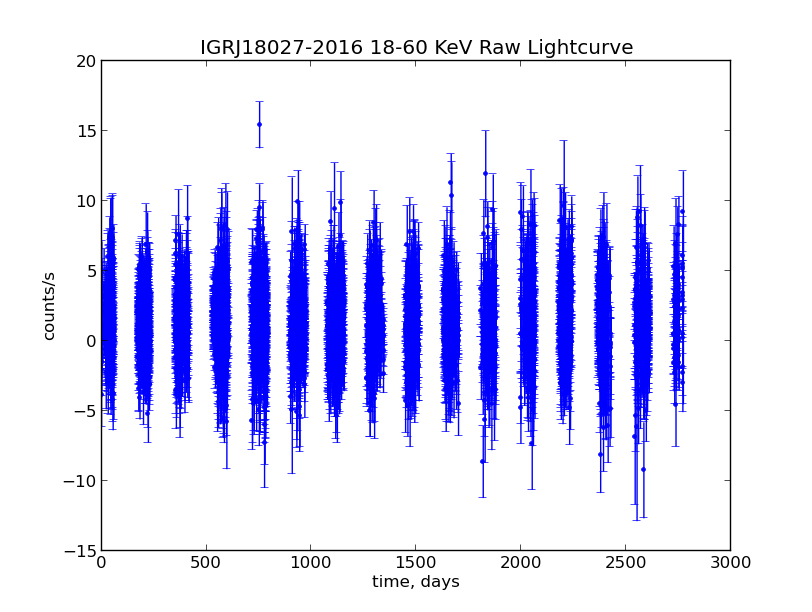
\includegraphics[width=130mm]{gfx/Fig1.png}
\caption{A raw lightcurve for the test source. Note the large errors on many data points.}
\label{Figure 1}
\end{figure}

\section{Re-binning the Data}
A simple tool for visualising the data is to be able to compile a graph of the entire light curve. However most sources from the archive have many thousands of individual science windows; the test source used had approximately 10,000. In order so that a sensible graph can be produced, the data shown needs to be cut down in a way that throws away as little useful information as possible. Re-binning collects groups of data points into a single data point. 

In the project code, a uniform bin size is selected, typically between 1 day to 1 month. Data points are grouped into the bins, and a flux measurement for each bin is calculated by taking an average of the members, weighted by the standard error. Furthermore, a new standard error is calculated for each bin by propagating errors through the calculation of the binned flux.

Re-binning the data is useful for visualising the data. However, a graph produced by re-binning the data will not show any variation in the source on a time period smaller than the bin size. Binning into one month bins loses all information that happens in the timescale of the orbital period of the object, which may be only a few days. This makes re-binning only a preliminary step in analysing a source. 

\begin{figure}[h!]
\centering
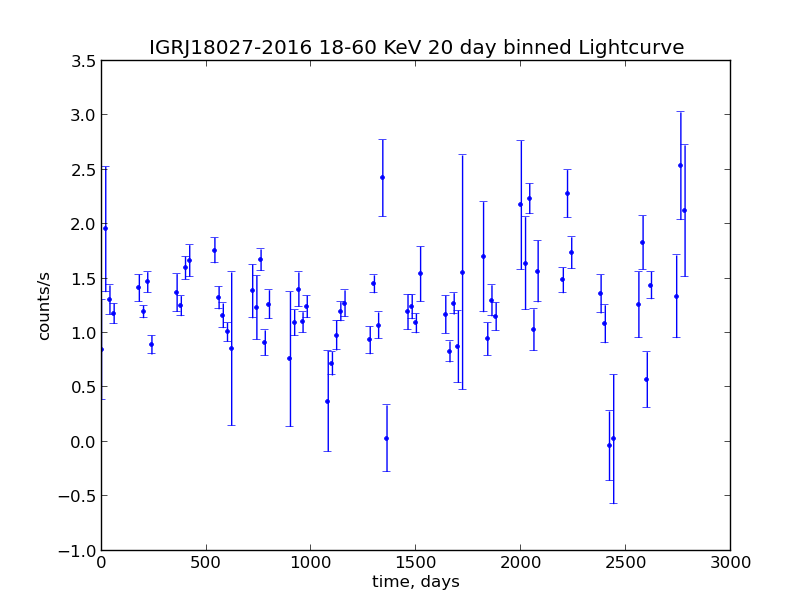
\includegraphics[width=130mm]{gfx/Fig2.png}
\caption{A re-binned light curve for the test source, with a 20 day bin size.}
\label{Figure 2}
\end{figure}

\ref{Figure 1} shows a raw lightcurve for the test source. Note the large errors on many data points. 
\ref{Figure 2} shows a re-binned light curve for the test source, with a 20 day bin size. Note that when only a few data points fall into a single bin, the bin can appear to have a large error. The points in the figure with the smallest error bars are typically calculated from many data points in the raw lightcurve.

\section{Finding Periodicities}
One of the key aims of the project is to find periodicities in the sample of sources, so it is necessary to have robust method to detect this within the data. One common method employed is to perform Fourier analysis. In breaking down the data into a series of sine waves, the periodic variations in flux will show up as the sine waves with the largest coefficients. However, Fourier analysis requires that the data points are evenly spaced, a criterion not often fulfilled in astronomy, and also not true of the INTEGRAL data.

\begin{figure}[h!]
\centering
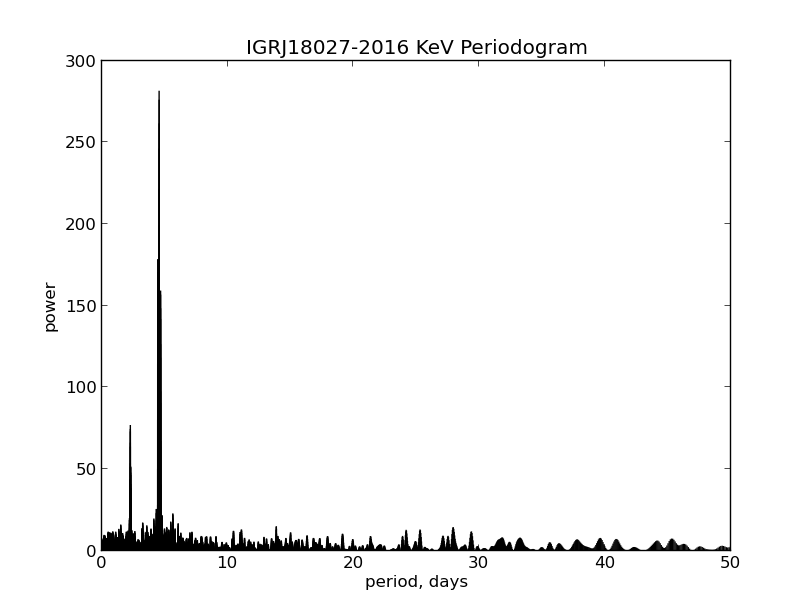
\includegraphics[width=130mm]{gfx/Fig3.png}
\caption{A periodogram for the test source, using the astropython implementation.}
\label{Figure 3}
\end{figure}

\subsection{Lomb-Scargle Method}
One alternative method, that this project uses, is the Lomb-Scargle method. This method fits trial sine waves to the data and then by minimising the squares of the residuals, produces a spectrum of the data. Crucially, the Lomb-Scargle Method can work on unevenly sampled data. 
There are two easily available implementations of the Lomb-Scargle method in python. One is available in Scipy 0.11 and another has been implemented by a contributor to astropython, which this project uses [ref]. Both implementations utilise Numpy, which has routines that are pre-compiled in C and Fortran, making the routine efficient.

Two useful outputs are produced from this section of the code. The first is the periodogram, which is a spectrum of the data. The test source is known to have a strong periodicity associated with an eclipse. This shows up clearly in the periodogram. Second, the Lomb-Scargle routine returns the highest peak in the periodogram, which corresponds to the strongest period. This is passed to the next section of the code for producing the folded light curves.

Whilst both routines perform the same overall function, the inner workings are a \textquotedblleft{}black box\textquotedblright{}. Experience showed that the astropython routine appeared to find a stronger peak, however there were exceptions where the Scipy implementation performed better. In general, the astropython implementation is shown, unless stated otherwise.

\begin{figure}[h!]
\centering
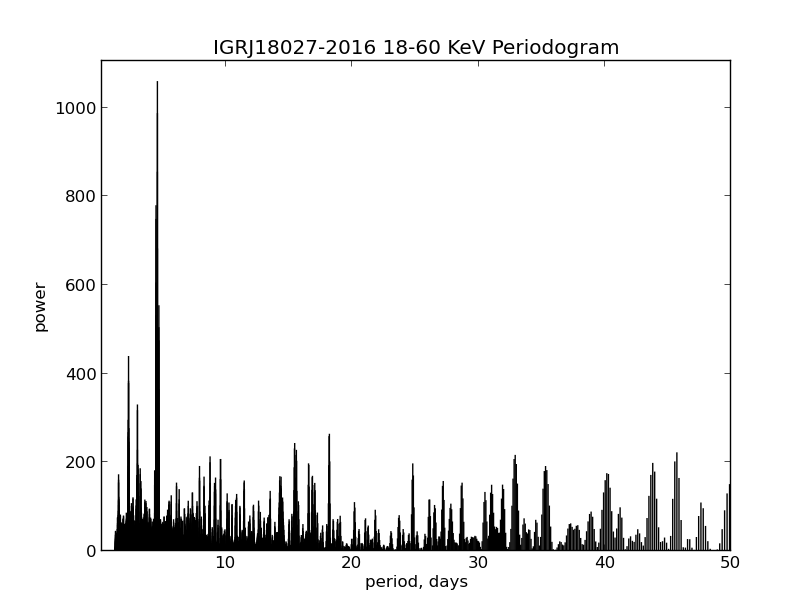
\includegraphics[width=130mm]{gfx/Fig4.png}
\caption{A periodogram for the test source, using the Scipy implementation.}
\label{Figure 4}
\end{figure}


\ref{Figure 3} shows a periodogram for the test source, using the astropython implementation. It shows a strong peak in power at approximately 4.6 days, which is due to the eclipse.
\ref{Figure 4} shows a periodogram for the test source, using the Scipy implementation. Whilst it also shows the same peak, it is obvious from inspection that the periodogram is more noisy.

\section{Folding the Lightcurve}
Using the period found from the Lomb-Scargle routine, the next step of the code is to produce a folded light curve. The light curve produced initially cannot reveal any significant amount of information about an object, since all variation is lost by re-binning the data. In the project code, by dividing each time coordinate by the period, and keeping only the remainder, the data is \textquotedblleft{}folded\textquotedblright{} on top of itself. This means that each identical point in the object\textquoteright{}s period will line up over each other. 

The next step is to define a set of bins, similar to the previous section, and to re-bin the folded data. Once again, a weighted average of the flux is taken, and errors calculated through. The number of bins is a trade-off. With a smaller number of bins, the averaging reduces the error on each measurement, however time resolution is lost. This can be seen in the test source, as each point of the eclipse occurs at the same place on the graph. Once averaged, the eclipse profile can be seen in the data, as the averaging process causes the points to converge to the true profile, and reduces the error greatly. 

\begin{figure}[h!]
\centering
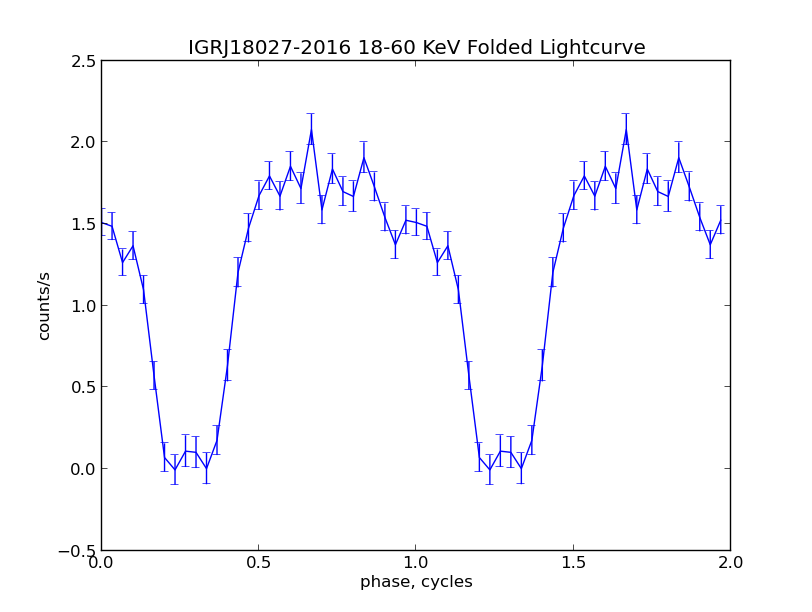
\includegraphics[width=130mm]{gfx/Fig5.png}
\caption{A folded and binned light curve, using the strongest peak from the periodogram, 4.570 days. Two cycles are shown for clarity.}
\label{Figure 5}
\end{figure}

\ref{Figure 5} shows the folded and binned light curve, using the strongest peak from the periodogram. Two cycles are shown for clarity. The eclipse shows through clearly, and the effect of the large data set reduces the size of the error bars significantly.

\subsection{Phase Dispersion Method}
Another means to detect periodicities in data is the Phase Dispersion Method. The Lomb-Scargle routine makes the implicit assumption that the signal in the data is sinusoidal, since all it fits are sine waves. This is a reasonable assumption when dealing with SGXBs such as the test source, and Cen X-3, since the eclipse is regular and the time of the eclipse forms a significant fraction of the folded light curve.  However, for sources such as BeXBs where the \textquotedblleft{}on time\textquotedblright{} of the sources is a very small fraction of the orbital period of the compact object, then this assumption breaks down. Sources that also have a high range, that flare particularly brightly also reduce the effectiveness of the Lomb-Scargle method. 
The Phase Dispersion Method makes no assumptions about the shape of the lightcurve. It works by attempting many trial folds of the data, and then binning the data down, where the process is the same that is used to produce the plot above. The key part of the method is that it compares the variance, or spread of points, within each bin to the variance of the entire data set as a whole. If a trial period is tested that is not a periodicity of the data, then the variance of points within a bin will on average be the same as the variance of the data as a whole. However if a trial period is tested that is a periodicity of the data, then the points within a bin will tend to cluster more tightly. This can be represented as a statistic for each trial fold, which tends to be $\simeq1$ for noise, and then reduces when a periodicity is found.

\begin{figure}[h!]
\centering
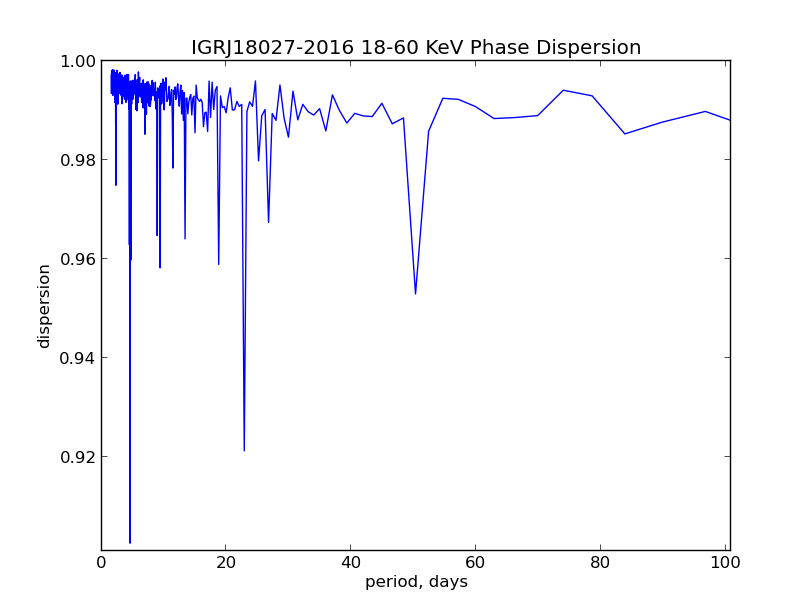
\includegraphics[width=130mm]{gfx/Fig6.png}
\caption{A PDM plot for the test source. Notice where the drop in the statistic coincides with the peak in the Lomb-Scargle periodogram, and the harmonics of the strongest frequency.}
\label{Figure 6}
\end{figure}

\ref{Figure 6} shows a PDM plot for the same test source. Notice where the drop in the statistic coincides with the peak in the Lomb-Scargle periodogram, and the harmonics of the strongest frequency.

Unfortunately, no PDM method already exists in any available python library, so this was coded from scratch. PAPER was used as a reference to code the method. This proved to be a technical challenge during the project. Furthermore, since the method is coded almost entirely in python, and due to the inherent nature of having to perform many trial folds of the data, the method is considerably slower to produce the same results as the Lomb-Scargle method. 

\section{Error calculations of the Lomb-Scargle Period}

When dealing with more challenging sources, it\textquoteright{}s useful to be able to quantify how accurate the period found by the Lomb-Scargle routine is. It\textquoteright{}s difficult to calculate errors conventionally, and also challenging to implement this in code. Two solutions were coded to be used in the project to find an error measurement. 

A Monte-Carlo simulation randomises the data. Each flux value is randomised according to a normal distribution with mean given by the flux and standard deviation given by its error. This generates a modified light curve which is processed by the Lomb-Scargle routine. The period is recorded, and the process repeated with a new randomised light curve generated from the original. Typically ten thousand runs are made as a minimum. A histogram of the periods is plotted, which should approximate a normal distribution with standard deviation that is the error on the original period.

Bootstrapping is another similar method. Rather than randomising the data, bootstrapping randomly discards data from the set. For N data points, N random integers between 1 and N are generated. Each integer corresponds to a data point, so that if the number X is generated, the Xth data point is copied to a new light curve. This allows for duplicate random integers, however the data point is only copied once. This reduced light curve is run through the routine, the period recorded, and a new light curve generated to repeat the process. 
 % Chapter 3
%% Chapter 4

\chapter{Results} % Chapter title

\label{ch:results} % For referencing the chapter elsewhere, use \autoref{ch:introduction} 

%----------------------------------------------------------------------------------------
\section{List of Sources}
Twenty two sources were analysed; a full list is shown below. Results have been grouped according to suggested class of HMXB, and approximately in order of confidence.
\begin{itemize}
\item 1A0535+262
\item AXJ1910.7+0917
\item Cen X-3
\item EXO2030+375
\item IGRJ08408-4503
\item IGRJ11215-5952
\item IGRJ16418-4532
\item IGRJ16465-4507
\item IGRJ16479-4514
\item IGRJ17391-3021
\item IGRJ17407-2808
\item IGRJ17544-2619
\item IGRJ18027-2016
\item IGRJ18219-1347
\item IGRJ18410-0535
\item IGRJ18450-0435
\item IGRJ18483-0311
\item MAXIJ1409-619
\item OAO1657-415
\item SAXJ1818.6-1703
\item Vela X-1
\item XPer
\end{itemize}
\clearpage{}

\section{Supergiant X-ray Binaries}
\subsection{Cen X-3}

\begin{figure}[h!]
\centering
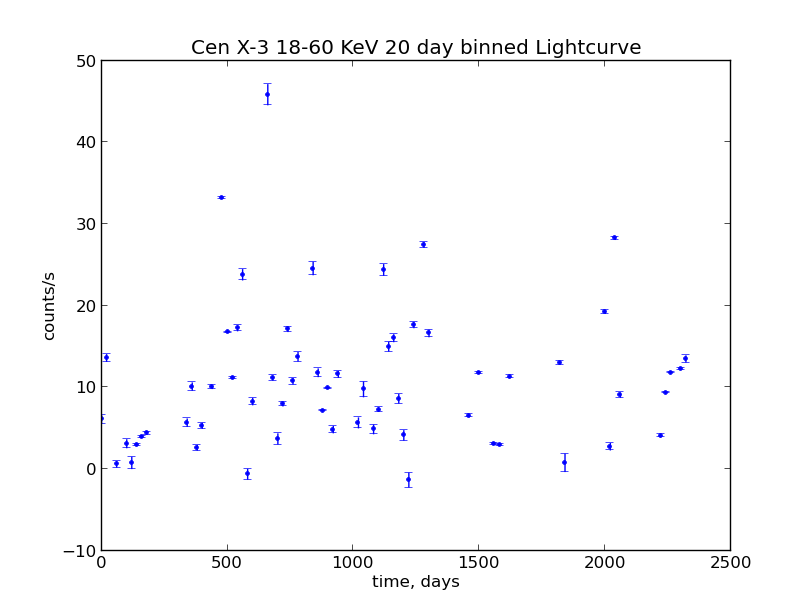
\includegraphics[width=130mm]{gfx/Fig7.png}
\caption{20 day binned lightcurve for Cen X-3.}
\label{Figure 7}
\end{figure}

Cen X-3 is a very bright and well studied source, and as it\textquoteright{}s designation would suggest, was one of the first X-ray sources to be discovered. It is a SGXB, and so is powered primarily by stellar wind loss. It has a well documented 2.087 day cycle.

\begin{figure}[h!]
\centering
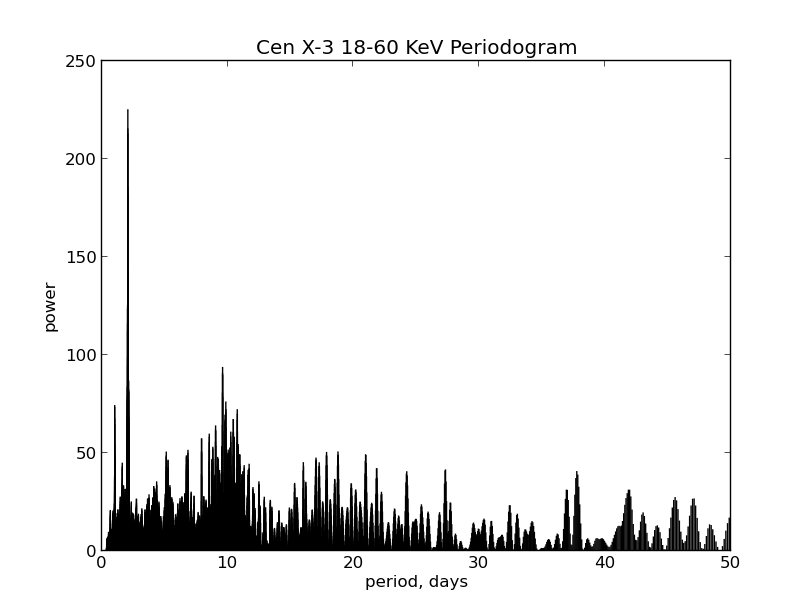
\includegraphics[width=130mm]{gfx/Fig8.png}
\caption{Periodogram for Cen X-3. The expected peak at 2.087 days is very clear.}
\label{Figure 8}
\end{figure}

\ref{Figure 7} shows a binned lightcurve. Although this does not reveal anything useful, it is an example of a particularly good source. Cen X-3 is very luminous, and the error bars and count rates reflect this. \ref{Figure 8} shows a periodogram from Cen X-3. The expected peak at 2.087 days is very clear. Once folded on this period, \ref{Figure 9} shows the eclipse profile. From these results, it is easy to see that Cen X-3 shows the behaviour expected of a SGXB. It is luminous and active except when eclipsing, and provides a good example to measure other less well known and more uncertain sources against. 

\begin{figure}[h!]
\centering
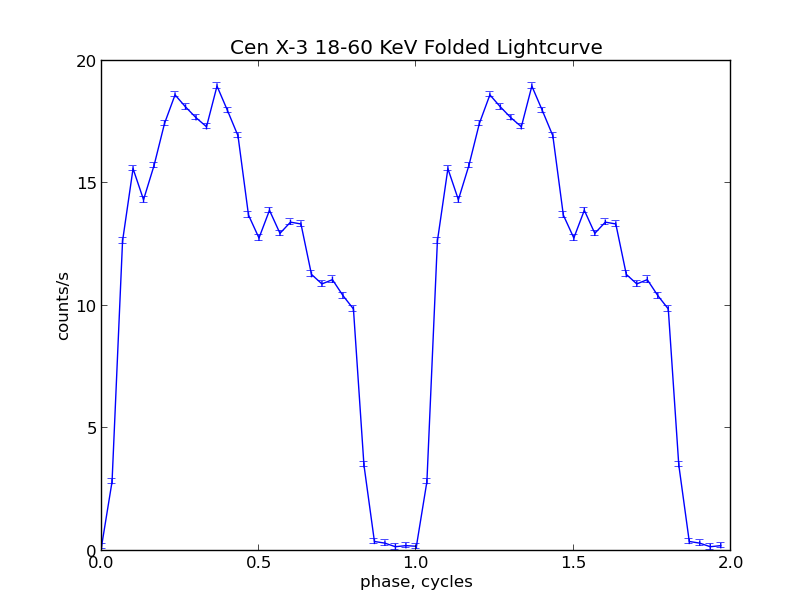
\includegraphics[width=130mm]{gfx/Fig9.png}
\caption{Folded lightcurve for Cen X-3.}
\label{Figure 9}
\end{figure} 

\clearpage
\subsection{Vela X-1}

\begin{figure}[h!]
\centering
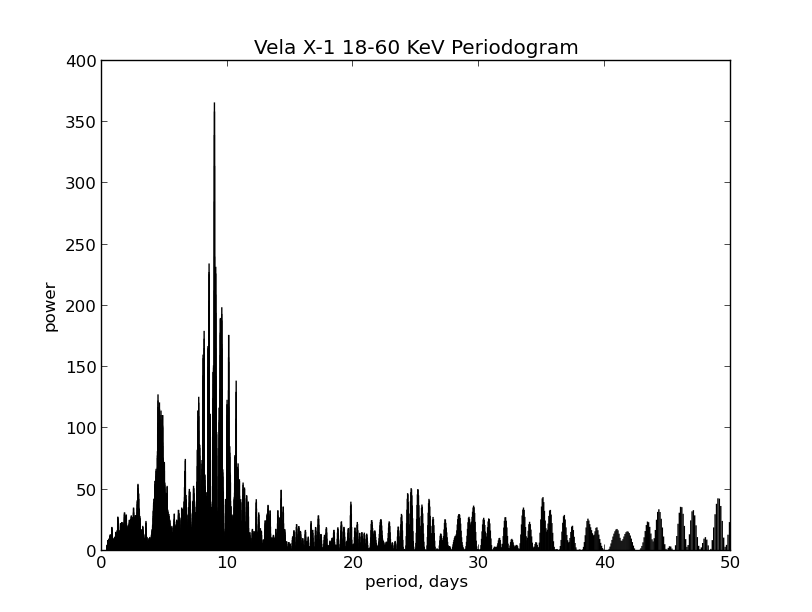
\includegraphics[width=130mm]{gfx/Fig10.png}
\caption{Periodogram for Vela X-1.}
\label{Figure 10}
\end{figure} 

Vela X-1 is another bright SGXB that was discovered early in the study of XRBs, and like Cen X-3 and Cyg X-1 could be considered a textbook example of it\textquoteright{}s class. The orbital period of the system is already known to be 8.964 days.

\ref{Figure 10} shows the periodogram, with a large peak at the expected 8.964 days. \ref{Figure 11} shows the folded light curve on that period, and the eclipse profile is shown convincingly. 

\begin{figure}[h!]
\centering
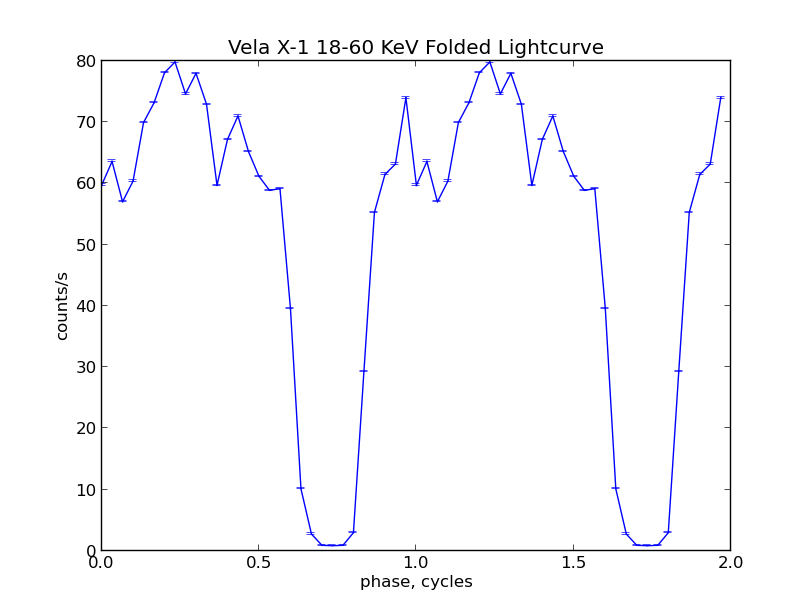
\includegraphics[width=130mm]{gfx/Fig11.png}
\caption{Folded lightcurve for Vela X-1. Period: 8.964 days.}
\label{Figure 11}
\end{figure} 

\subsection{OAO1657-415}
OAO1657-415 is very similar to both Vela X-1 and Cen X-3, and is another SGXB. It has a slightly longer known period of 10.4 days and it has been suggested that this source might not be entirely wind-fed, and that a proportion of the accretion may be through a disk. These results corroborate with the 10.4 day period, as shown in the periodogram \ref{Figure 12}, which peaks at 10.45 days. \ref{Figure 13} shows the folded lightcurve, and the eclipse, clearly showing that these results agree with the body of literature. 

\begin{figure}[h!]
\centering
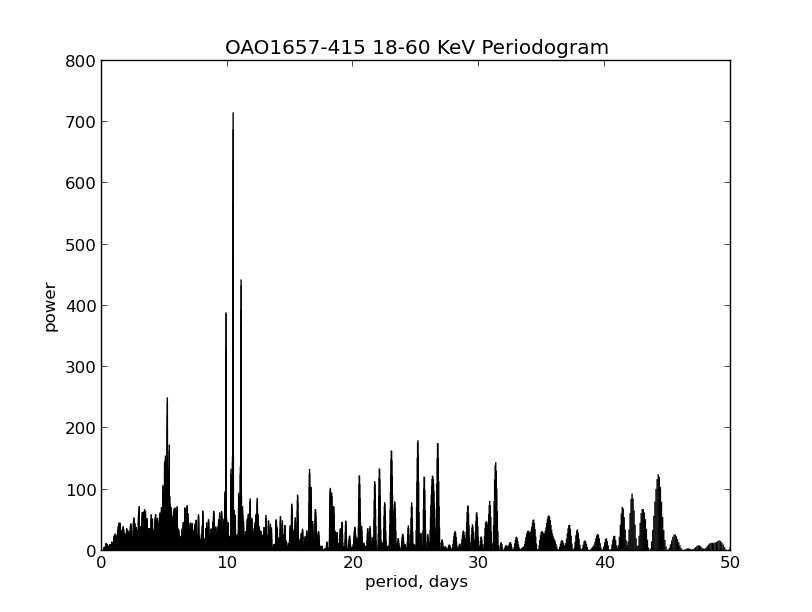
\includegraphics[width=130mm]{gfx/Fig12.png}
\caption{Periodogram for OAO1657-415. Peak at 10.45 days.}
\label{Figure 12}
\end{figure} 

\begin{figure}[h!]
\centering
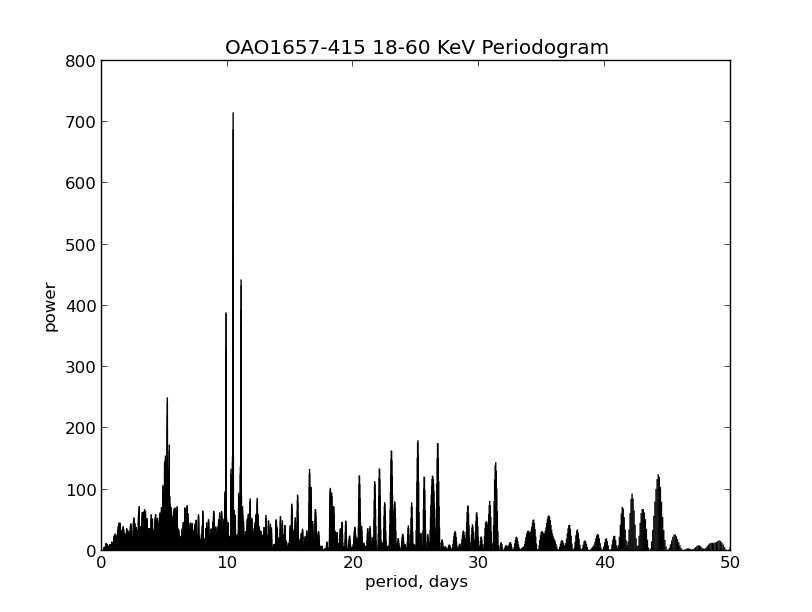
\includegraphics[width=130mm]{gfx/Fig12.png}
\caption{Folded lightcurve for OAO1657-415. Period: 10.45 days.}
\label{Figure 13}
\end{figure} 

\subsection{IGRJ18027-2016}
IGRJ18027-2016 is another probable Supergiant X-ray Binary, and was the test source used in this project. The results for this source were shown in the previous section. \ref{Figure 3} shows the periodogram, and \ref{Figure 5} shows the folded light curve and eclipse, with a period of 4.570 days. 

\clearpage

 % Chapter 4 - empty template

%----------------------------------------------------------------------------------------
%	THESIS CONTENT - APPENDICES
%----------------------------------------------------------------------------------------

\appendix

\part{Appendix} % New part of the thesis for the appendix

% Appendix A

\chapter{Appendix Test}

%----------------------------------------------------------------------------------------

\lipsum[13-14]

%----------------------------------------------------------------------------------------

\section{Appendix Section Test}
\lipsum[15]

\graffito{More dummy text}
\lipsum[16]

%----------------------------------------------------------------------------------------

\section{Another Appendix Section Test}
\lipsum[17]

\begin{table}
\myfloatalign
\begin{tabularx}{\textwidth}{Xll} \toprule
\tableheadline{labitur bonorum pri no} & \tableheadline{que vista}
& \tableheadline{human} \\ \midrule
fastidii ea ius & germano &  demonstratea \\
suscipit instructior & titulo & personas \\
\midrule
quaestio philosophia & facto & demonstrated \\
\bottomrule
\end{tabularx}
\caption[Autem usu id]{Autem usu id.}
\label{tab:moreexample}
\end{table}

\lipsum[18]

\begin{lstlisting}[float,caption=A floating example]
for i:=maxint to 0 do
begin
{ do nothing }
end;
\end{lstlisting} % Appendix A
%% Appendix X

\chapter{Appendix Title}

%----------------------------------------------------------------------------------------

% Content begins here % Appendix B - empty template

%----------------------------------------------------------------------------------------
%	POST-CONTENT THESIS PAGES
%----------------------------------------------------------------------------------------

\cleardoublepage% Bibliography

\label{app:bibliography} % Reference the bibliography elsewhere with \autoref{app:bibliography}

\manualmark
\markboth{\spacedlowsmallcaps{\bibname}}{\spacedlowsmallcaps{\bibname}} 
\refstepcounter{dummy}

\addtocontents{toc}{\protect\vspace{\beforebibskip}} % Place the bibliography slightly below the rest of the document content in the table of contents
\addcontentsline{toc}{chapter}{\tocEntry{\bibname}}

\bibliographystyle{plainnat}

\bibliography{FrontBackMatter/Bibliography}

\begin{thebibliography}{99}

\bibitem{simbad}
SIMBAD Astronomical Database, http://simbad.u-strasbg.fr/simbad/

\bibitem{Masetti}
Masetti, N., Mason, E.,  Morelli, L., et al., Unveiling the nature of INTEGRAL objects through optical spectroscopy, Astronomy & Astrophysics, no. 482, pg. 113-132 (2008).

\bibitem{Mason}
Mason, A.B., Norton A.J., et al., The masses of the neutron and donor star in the high-mass X-ray binary IGR J18027-2016, Astronomy & Astrophysics, no. 532, Article 124 (2011).

\bibitem{Seward}
Seward, F.D. and Charles, P.A., Exploring the X-ray Universe, Cambridge University Press, ISBN 978-0521884839

\bibitem{Goldwurm}
Goldwurm A. et. al, Gamma-Ray Imaging with the Coded Mask IBIS Telescope, http://arxiv.org/abs/astro-ph/0102386, February 2001

\bibitem{Sidoli}
Sidoli, L. et. al., The XMM–Newton view of supergiant fast X-ray transients: the case of IGR J16418-4532, Monthly Notices of the Royal Astronomical Society, Vol 420, Issue 1, pages 554-561, February 2012

\bibitem{Romano}
Romano, P. et. al., Swift/X-ray Telescope monitoring of the candidate supergiant fast X-ray transient IGR J16418-4532, Monthly Notices of the Royal Astronomical Society Volume 419, Issue 3, pages 2695-2702, January 2012


\end{thebibliography} % Bibliography

\cleardoublepage% Colophon (a brief description of publication or production notes relevant to the edition)

\pagestyle{empty}

\hfill

\vfill

\pdfbookmark[0]{Colophon}{colophon}

\section*{Colophon}

This document was typeset using the typographical look-and-feel \texttt{classicthesis} developed by Andr\'e Miede. The style was inspired by Robert Bringhurst's seminal book on typography ``\emph{The Elements of Typographic Style}''. \texttt{classicthesis} is available for both \LaTeX\ and \mLyX: 

\begin{center}
\url{http://code.google.com/p/classicthesis/}
\end{center}

\noindent Happy users of \texttt{classicthesis} usually send a real postcard to the author, a collection of postcards received so far is featured here: 

\begin{center}
\url{http://postcards.miede.de/}
\end{center}
 
\bigskip

\noindent\finalVersionString % Colophon

\cleardoublepage% Declaration

\refstepcounter{dummy}
\pdfbookmark[0]{Declaration}{declaration} % Bookmark name visible in a PDF viewer

\chapter*{Declaration} % Declaration section text

\thispagestyle{empty}

Put your declaration here.
\bigskip
 
\noindent\textit{\myLocation, \myTime}

\smallskip

\begin{flushright}
\begin{tabular}{m{5cm}}
\\ \hline
\centering\myName, \today \\
\end{tabular}
\end{flushright}
 % Declaration

%----------------------------------------------------------------------------------------

\end{document}
